\documentclass[compress, darktitle, framenumber]{beamer}
\usepackage{pgfplots}
\usepackage{tikz}
\usepackage{xparse}
\usepackage{graphicx}
\usepackage{epsfig}
\usepackage{float}
\restylefloat{figure}
\restylefloat{table}
\usepackage[font=small,format=plain,labelfont=bf,up,textfont=it,up]{caption}

\usepackage[dutch]{babel}
\usepackage{enumerate}

%\usepackage[usenames,dvipsnames]{color}

\usepackage{amsmath,amsfonts,amsthm,amssymb}
\usepackage{mathrsfs}
\usepackage{mathtools}
\usepackage{accents}
\usetikzlibrary{matrix,arrows}

\mathtoolsset{showonlyrefs}

\usetheme{UniversiteitAntwerpen}

\title{Wisku$\mathbb{N}$de in-$\mathbb{Z}$icht}
\subtitle{Wiskunde in muziek}
\author{Pieter Belmans (\texttt{pieter.belmans@uantwerpen.be}) \\ Matthias Roels (\texttt{matthias.roels@uantwerpen.be})}
\date{9 januari 2014}

%%%%%%%%%%%%%%%%%%%%%%%%%%%%%%%%%%%
%%%%%%%%%%Commando's Matthias%%%%%%%%%

\newcommand{\comm}[1]{\lbrack #1 \rbrack} %notatie van Lie haak
\newcommand{\set}[1]{\left\{ #1 \right\} } %notatie voor haakjes voor een verzameling
\newcommand{\brac}[1]{\left( #1 \right)} %notatie voor haakjes

\newcommand{\R}{\mathbb{R}} % the field of the reals
\newcommand{\N}{\mathbb{N}} % the field of the natural numbers
\newcommand{\C}{\mathbb{C}} % the field of complex number
\newcommand{\Z}{\mathbb{Z}} % the field of integers

\AtBeginSection[]
{
  \begin{frame}<beamer>
    \frametitle{Overzicht}
    \tableofcontents[currentsection]
  \end{frame}
}



\begin{document}
\begin{frame}
  \titlepage
\end{frame}

\section{Inleiding}


\begin{frame}
\frametitle{Wat is geluid}
\begin{itemize}
\item Geluid is een periodisch signaal (een ``golf '') 
\item Wiskundig: een functie die afhangt van de tijd zodat $$f(t+P)=f(t),$$ met $P$ de periode.
\end{itemize}
\begin{alertblock}{Vraag:}
Hoe beschrijft men deze functies? 
\end{alertblock}
\end{frame}

\begin{frame}
\frametitle{Wat zijn de meest eenvoudige signalen?}
\begin{itemize}
\item Dit zijn de zgn. goniometrische functies $$f(t)=A\cos (\omega t) \quad \text{en} \quad g(t)=B\sin (\omega t),$$ met $A$ en $B$ de amplitude en $\omega$ de frequentie. 
\item Amplitude: $\frac{1}{2}$(het verschil tussen piek en dal)
\item Frequentie: $($afstand tussen twee toppen van de golf$)^{-1}$
\end{itemize}
\begin{alertblock}{Vraag:}
Hoe klinkt zo'n signaal? \\
Kunnen we deze gebruiken om complexere signalen te beschrijven?  
\end{alertblock}
\end{frame}

\begin{frame}
\frametitle{Sinusgolf}
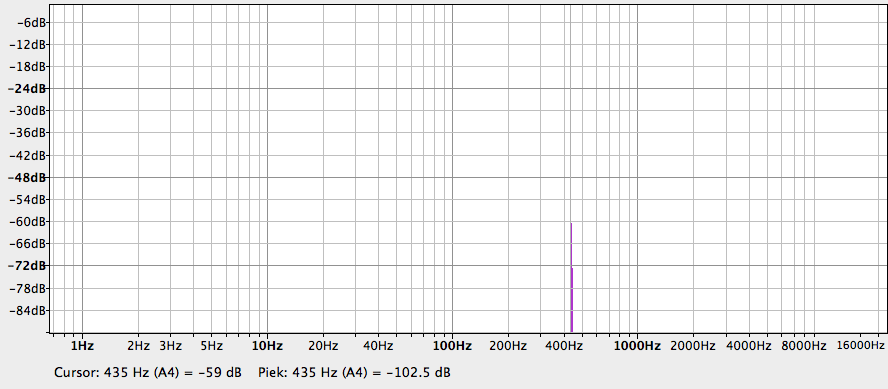
\includegraphics[width=\textwidth]{Sin_wave.png}
\begin{block}{Audiofragment}
\texttt{Sin\_wave.aup}
\end{block}
\end{frame}

\begin{frame}[fragile]
\frametitle{Een analogie met vectoren}
\begin{itemize}
\item Een vector kan geschreven worden als $\vec{v}=a\vec{e}_x+b\vec{e}_y.$
\end{itemize}
\begin{tikzpicture}[scale=1.5]
    % Draw axes
    \draw [>=stealth,<->,thick] (0,2.5) node (yaxis) [above] {$y$}
        |- (3,0) node (xaxis) [right] {$x$};
    % Draw two intersecting lines
    \draw[uared!80, ultra thick, >=stealth,->] (0,0) coordinate (a_1) -- (2,1.8) node[midway, left]{$\vec{v}$} coordinate (c);
    % Draw lines indicating intersection with y and x axis. Here we use
    % the perpendicular coordinate system
    \draw[dashed] (yaxis |- c) node[left] {$b$}
        -| (xaxis -| c) node[below] {$a$};
\end{tikzpicture}
\begin{itemize}
\item We willen iets gelijkaardigs doen met signalen: deze schrijven als lineaire combinaties van ``basisfuncties.''
\end{itemize}
\end{frame}

\begin{frame}
\frametitle{Fourierreeksen}
\begin{itemize}
\item periodische signalen ontbinden in (mogelijk oneindige) som van eenvoudige signalen 
$$f(t)=\frac{A_0}{2}+\sum_{n=0}^{\infty}\brac{A_n \cos(\omega_n t)+B_n\sin(\omega_n t)}. $$
\item oneindige som mag niet oneindig geven. \\ \noindent 
$\implies$ amplitudes $A_n$ en $B_n$ zullen kleiner en kleiner worden naarmate $n$ groter wordt. 
\end{itemize}
\end{frame}


\begin{frame}
  \frametitle{Blokgolf}
  \centering
  \begin{tikzpicture}
    \begin{axis}[
      domain = 0:6*pi,
      width = \textwidth,
      height = \textheight*.8,
      smooth,
      no markers,
      samples = 20,
      xtick = {0,3.1415,...,18.8495},
      xticklabels={$0$,$\pi$,$2\pi$,$3\pi$,$4\pi$,$5\pi$,$6\pi$},
      xlabel = {$t$},
    ]
      \only<2-3>{\addplot[vividbrown] {sin(deg(1*x))/1};}

      \only<3-4>{\addplot[uared!50] {sin(deg(3*x))/3};}
      \only<4-5>{\addplot[vividbrown] {sin(deg(1*x))/1+sin(deg(3*x))/3};}

      \only<5-6>{\addplot[uared!50] {sin(deg(5*x))/5};}
      \only<6-7>{\addplot[vividbrown] {sin(deg(1*x))/1+sin(deg(3*x))/3+sin(deg(5*x))/5};}

      \only<7-8>{\addplot[uared!50] {sin(deg(7*x))/7};}
      \only<8-9>{\addplot[vividbrown] {sin(deg(1*x))/1+sin(deg(3*x))/3+sin(deg(5*x))/5+sin(deg(7*x))/7};}

      \addplot[const plot, thick] coordinates {(0,0) (0,1) (pi,1) (pi,-1) (2*pi,-1) (2*pi,1) (3*pi,1) (3*pi,-1) (4*pi,-1) (4*pi,1) (5*pi,1) (5*pi,-1) (6*pi,-1) (6*pi,0)};
    \end{axis}
  \end{tikzpicture}
\end{frame}


\begin{frame}
\frametitle{Blokgolf (2)}
\centering
\begin{tikzpicture}[x={(1cm,0.5cm)},z={(0cm,0.5cm)},y={(1cm,-0.2cm)}]
\draw[->,thick,black!70] (0,6.5,0) -- (3.8,6.5,0) node[above left] {Frequentie};
\draw[->,thick,black!70] (0,0,0) -- (0,6.5,0) node[below right] {Tijd};
\draw[->,thick] (0,0,0) -- (0,0,2) node[above] {Amplitude};
\foreach \y in {0.5,1.5,...,3.5}{
\draw [cyan!50, domain=0:2*pi,samples=20,smooth] 
 plot (\y,\x, {sin(4*\y*\x r)/\y });
\draw[blue, ultra thick] (\y,6.5,0) -- (\y,6.5,1/\y);
}
\draw [uared, thick, domain=0:2*pi,samples=20,smooth] 
plot (0,\x, {sin(4*0.5*\x r)/0.5 + sin(4*1.5*\x r)/1.5 + sin(4*2.5*\x r)/2.5 + sin(4*3.5*\x r)/3.5 + sin(4*4.5*\x r)/4.5 + sin(4*5.5*\x r)/5.5} );
\end{tikzpicture}
\end{frame}

\begin{frame}
\frametitle{Blokgolf (3)}
Vorige slide: grafische weergave van eerste 4 termen van fourierreeks:
\begin{equation}
s(x)\approx\sin{(t)}+\frac{1}{\pi}\sin{(2t)}+\frac{2}{3\pi}\sin{(3t)}-
\frac{1}{2\pi}\sin{(4t)}.
\end{equation}
\begin{block}{Opmerking:}
Dit is slechts een benadering! Deze wordt beter en beter naarmate er meer termen worden toegevoegd.
\end{block}
\end{frame}

\begin{frame}
\frametitle{Blokgolf (4)}
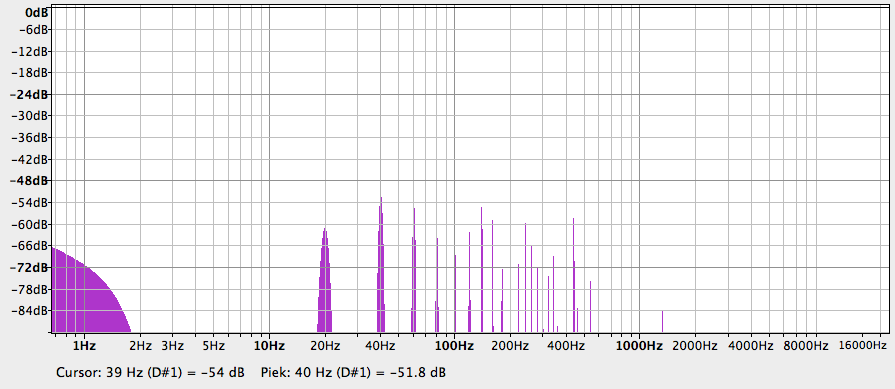
\includegraphics[width=\textwidth]{Square_wave.png}
\begin{block}{Audiofragment:}
\texttt{Square\_wave.aup} 
\end{block} 
\end{frame}


\begin{frame}
  \frametitle{Zaagtand golf}
 \centering
  \begin{tikzpicture}
    \begin{axis}[
      domain = 0:6*pi,
      width = \textwidth,
      height = \textheight*.8,
      smooth,
      no markers,
      samples = 20,
      xtick = {0,3.1415,...,18.8495},
      xticklabels={$0$,$\pi$,$2\pi$,$3\pi$,$4\pi$,$5\pi$,$6\pi$},
      xlabel = {$t$},
    ]
      \only<2-3>{\addplot[vividbrown] {2/pi*sin(deg(1*x))/1};}

      \only<3-4>{\addplot[uared!50] {-2/pi*sin(deg(2*x))/2};}
      \only<4-5>{\addplot[vividbrown] {2/pi*sin(deg(1*x))/1-2/pi*sin(deg(2*x))/2};}

      \only<5-6>{\addplot[uared!50] {2/pi*sin(deg(3*x))/3};}
      \only<6-7>{\addplot[vividbrown] {2/pi*sin(deg(1*x))/1-2/pi*sin(deg(2*x))/2+2/pi*sin(deg(3*x))/3};}

      \only<7-8>{\addplot[uared!50] {-2/pi*sin(deg(4*x))/4};}
      \only<8-9>{\addplot[vividbrown] {2/pi*sin(deg(1*x))/1-2/pi*sin(deg(2*x))/2+2/pi*sin(deg(3*x))/3-2/pi*sin(deg(4*x))/4};}

    \addplot[sharp plot, thick] coordinates {(0,0)(pi,1) (pi,-1) (3*pi,1) (3*pi,-1) (5*pi,1) (5*pi,-1) (6*pi,0)};
    \end{axis}
  \end{tikzpicture}
\end{frame}

\begin{frame}
\frametitle{Zaagtand golf (2)}
Vorige slide: grafische weergave van eerste 4 termen van fourierreeks:
\begin{equation}
s(x)\approx\frac{2}{\pi}\sin{(t)}-\frac{1}{\pi}\sin{(2t)}+\frac{2}{3\pi}\sin{(3t)}-
\frac{1}{2\pi}\sin{(4t)}.
\end{equation}
\begin{block}{Opmerking:}
Ook hier geldt: Benadering wordt beter en beter naarmate er meer termen worden toevoegen.
\end{block}
\end{frame}

\begin{frame}
\frametitle{Zaagtand golf (3)}
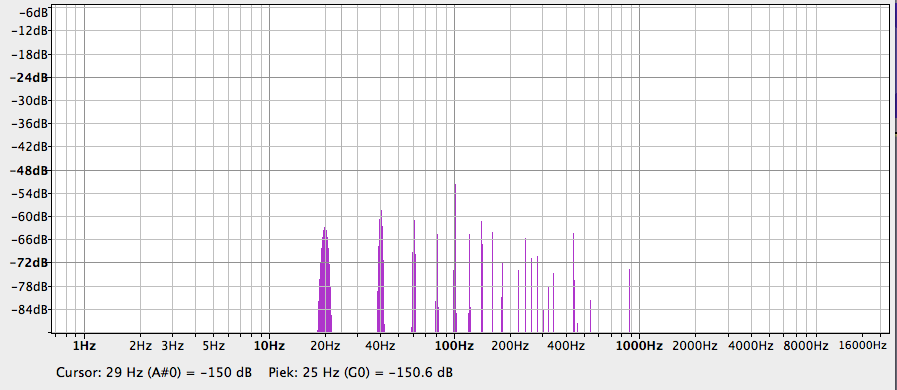
\includegraphics[width=\textwidth]{Sawtooth_wave.png}
\begin{block}{Audiofragment:}
\texttt{Sawtooth\_wave.aup}
\end{block}
\end{frame}

\section{Gitaar fragmenten}

\begin{frame}
\frametitle{Hoe ontstaat gitaargeluid?}
\begin{itemize}
\item Trilling van snaren wordt omgezet in wisselspanning door magnetische spoel: \textit{de pickups}. (Wet van Faraday-Lenz)
\item Wisselspanning moet versterkt worden om via luidsprekers hoorbare klank op te leveren. 
\item Meest courant: versterking via vacu\"umbuizen omwille van unieke klank.
\item Inputspanning van buis begrensd door minimum (z'n voeding) en maximum (op voorhand ingesteld: \textit{bias spanning}).
\item Binnen deze grenzen: versterking lineair, d.w.z. elke frequentie in het signaal wordt op dezelfde manier versterkt. 
\item Levert Cleane gitaarklank. 
\end{itemize}
\end{frame}

\begin{frame}
\frametitle{Versterking van gitaargeluid}
\begin{alertblock}{Vraag:}
Wat gebeurd er wanneer de inputspanning de maximumspanning nadert?
\end{alertblock}
\begin{itemize}
\item Versterking niet-lineair: kleinere spanningen worden (relatief gezien) meer versterkt dan grotere.
\item Toppen van de golf worden afgerond: \textit{Overdrive} of \textit{Clipping}.
\item Boventonen even veelvoud van grondto(o)n(en): vollere en warmere klank!
\item Distortion: Golftoppen worden afgekapt $\rightarrow$ vreemde componenten in spectrum
\item Clipping levert typische rocksound.
\end{itemize}
\end{frame}

\begin{frame}
\frametitle{Versterking van gitaargeluid(2)}
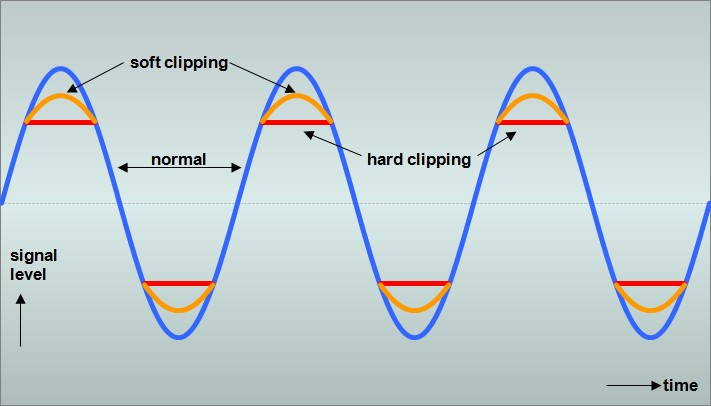
\includegraphics[width=\textwidth]{clipping.png}
\end{frame}

\begin{frame}
\frametitle{\'e\'en enkele noot}
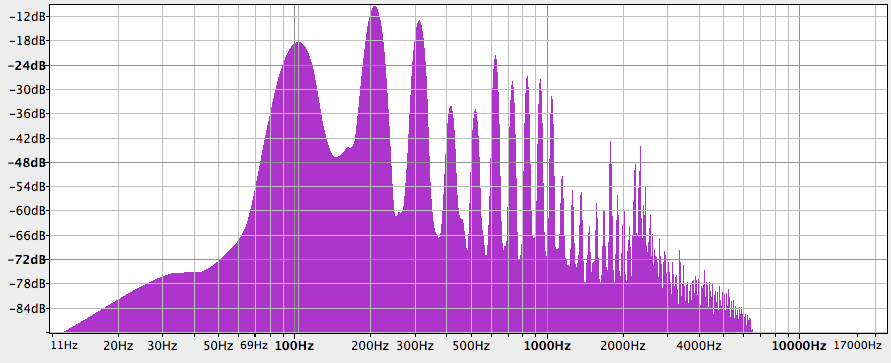
\includegraphics[width=\textwidth]{A-flat.png}
\begin{block}{Audiofragment:}
\texttt{A-flat-note.aup} 
\end{block}
\end{frame}

\begin{frame}
\frametitle{\'e\'en enkele noot(2)}
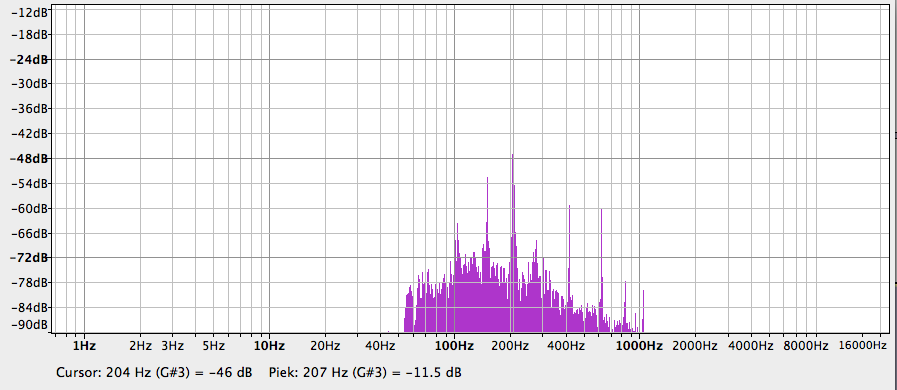
\includegraphics[width=\textwidth]{A-flat-harmonic.png}
\begin{block}{Audiofragment:}
\texttt{A-flat-harmonic.aup} 
\end{block}
\end{frame}

\begin{frame}
\frametitle{\'e\'en enkele noot: conclusie}
\begin{itemize}
\item Grondnoot is in beide gevallen duidelijk herkenbaar.
\item Harmoniek: boventonen altijd dubbel van grondfrequentie. 
\item Zuivere noot: andere boventonen die typische klankkleur van gitaar vormen. 
\item Kleinere schijnbaar onverklaarbare pieken door discretisatie van signaal. 
\end{itemize}
\end{frame}


\begin{frame}
\frametitle{C-noot}
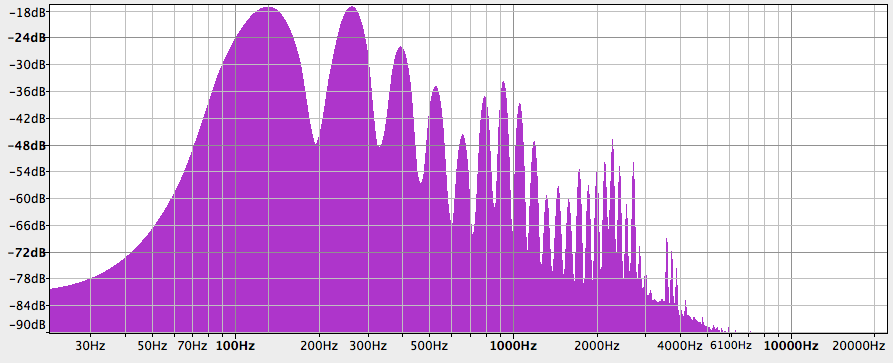
\includegraphics[width=\textwidth]{C-note.png}
\begin{block}{Audiofragment:}
\texttt{C-note.aup} 
\end{block}
\end{frame}


\begin{frame}
\frametitle{C-Akkoord}
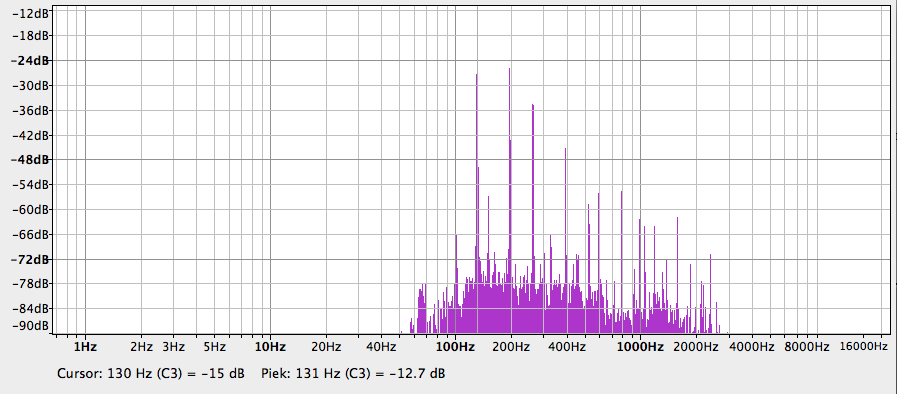
\includegraphics[width=\textwidth]{C-powerchord.png}
\begin{block}{Audiofragment:}
\texttt{C-powerchord.aup}
\end{block}
\end{frame}

\begin{frame}
\frametitle{C-Akkoord (2)}
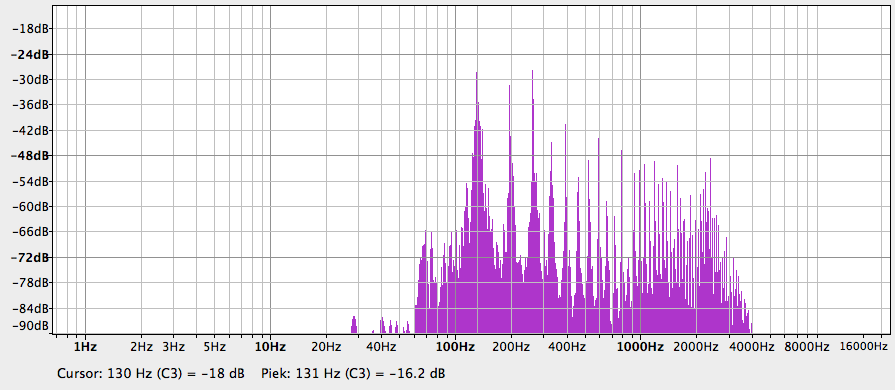
\includegraphics[width=\textwidth]{C-powerchord-overdriven.png}
\begin{block}{Audiofragment:}
\texttt{C-powerchord-overdriven.aup}
\end{block}
\end{frame}

\begin{frame}
\frametitle{C-Akkoord (3)}
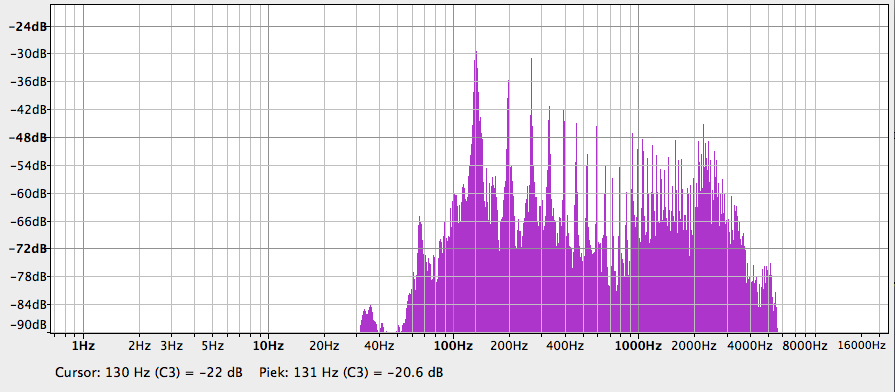
\includegraphics[width=\textwidth]{C-powerchord-heavily-distorted.png}
\begin{block}{Audiofragment:}
\texttt{C-powerchord-heavily-distorted.aup} 
\end{block}
\end{frame}

\begin{frame}
\frametitle{Conclusie: Clipping}
\begin{itemize}
\item Clean: akkoordnoten duidelijk terug te vinden. 
\item Effect van clipping duidelijk zichtbaar in spectra!
\end{itemize}
\end{frame}

\begin{frame}
\frametitle{C-Akkoord (4)}
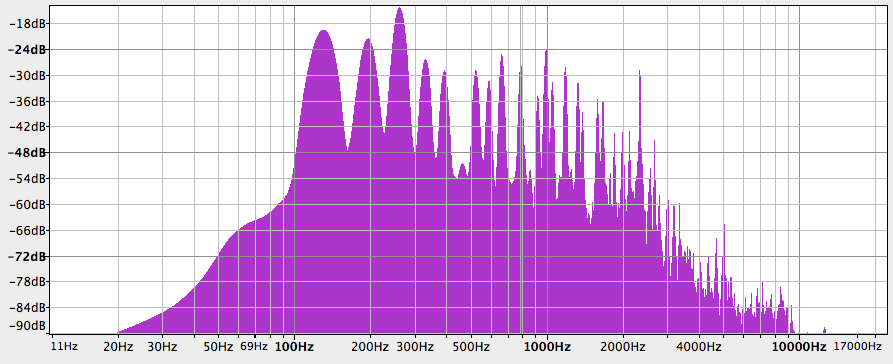
\includegraphics[width=\textwidth]{C-major-chord.png}
\begin{block}{Audiofragment:}
\texttt{C-major-chord.aup} 
\end{block}
\end{frame}


\begin{frame}
\frametitle{Extra}
\begin{block}{Audiofragment:}
\texttt{F-sharp-chord.aup} \\
\texttt{F-sharp-chord-overdriven.aup} \\
\end{block}
\end{frame}

\begin{frame}
\begin{center}
\huge
Bedankt voor jullie aandacht \\[1cm]
\Large
Zijn er nog vragen?
\end{center}
\end{frame}

\end{document}

